\documentclass[titlepage, 12pt]{article}

\usepackage{framed}
\usepackage{enumitem}
\usepackage{geometry}
\geometry{
  letterpaper,
  margin=1in,
}

\usepackage{graphicx}
\graphicspath{{./images/}}
\usepackage{hyperref}
\usepackage{float}
% \usepackage{subcaption}
\usepackage{amssymb}

\title{SE 2XB3 Group 4 Report 8}
\author{
  Huang, Kehao \\
  400235182 \\
  \texttt{huangk53@mcmaster.ca} \\
  L01
  \and
  Jiao, Anhao \\
  400251837 \\
  \texttt{jiaoa3@mcmaster.ca} \\
  L01
  \and
  Ye, Xunzhou \\
  400268576 \\
  \texttt{yex33@mcmaster.ca} \\
  L01
}
\date{23 March 2021}

\begin{document}
\maketitle{}

\newpage{}

\section{Prim vs Prim}

We experimented with the empirical run times of Prim v1 and Prim v2 on randomly
generated and connected graphs of size 100 to 1000. As expected, Prim v2 is much
faster than v1 as shown in Figure \ref{fig:comp}.
\begin{figure}[h]
  \centering
  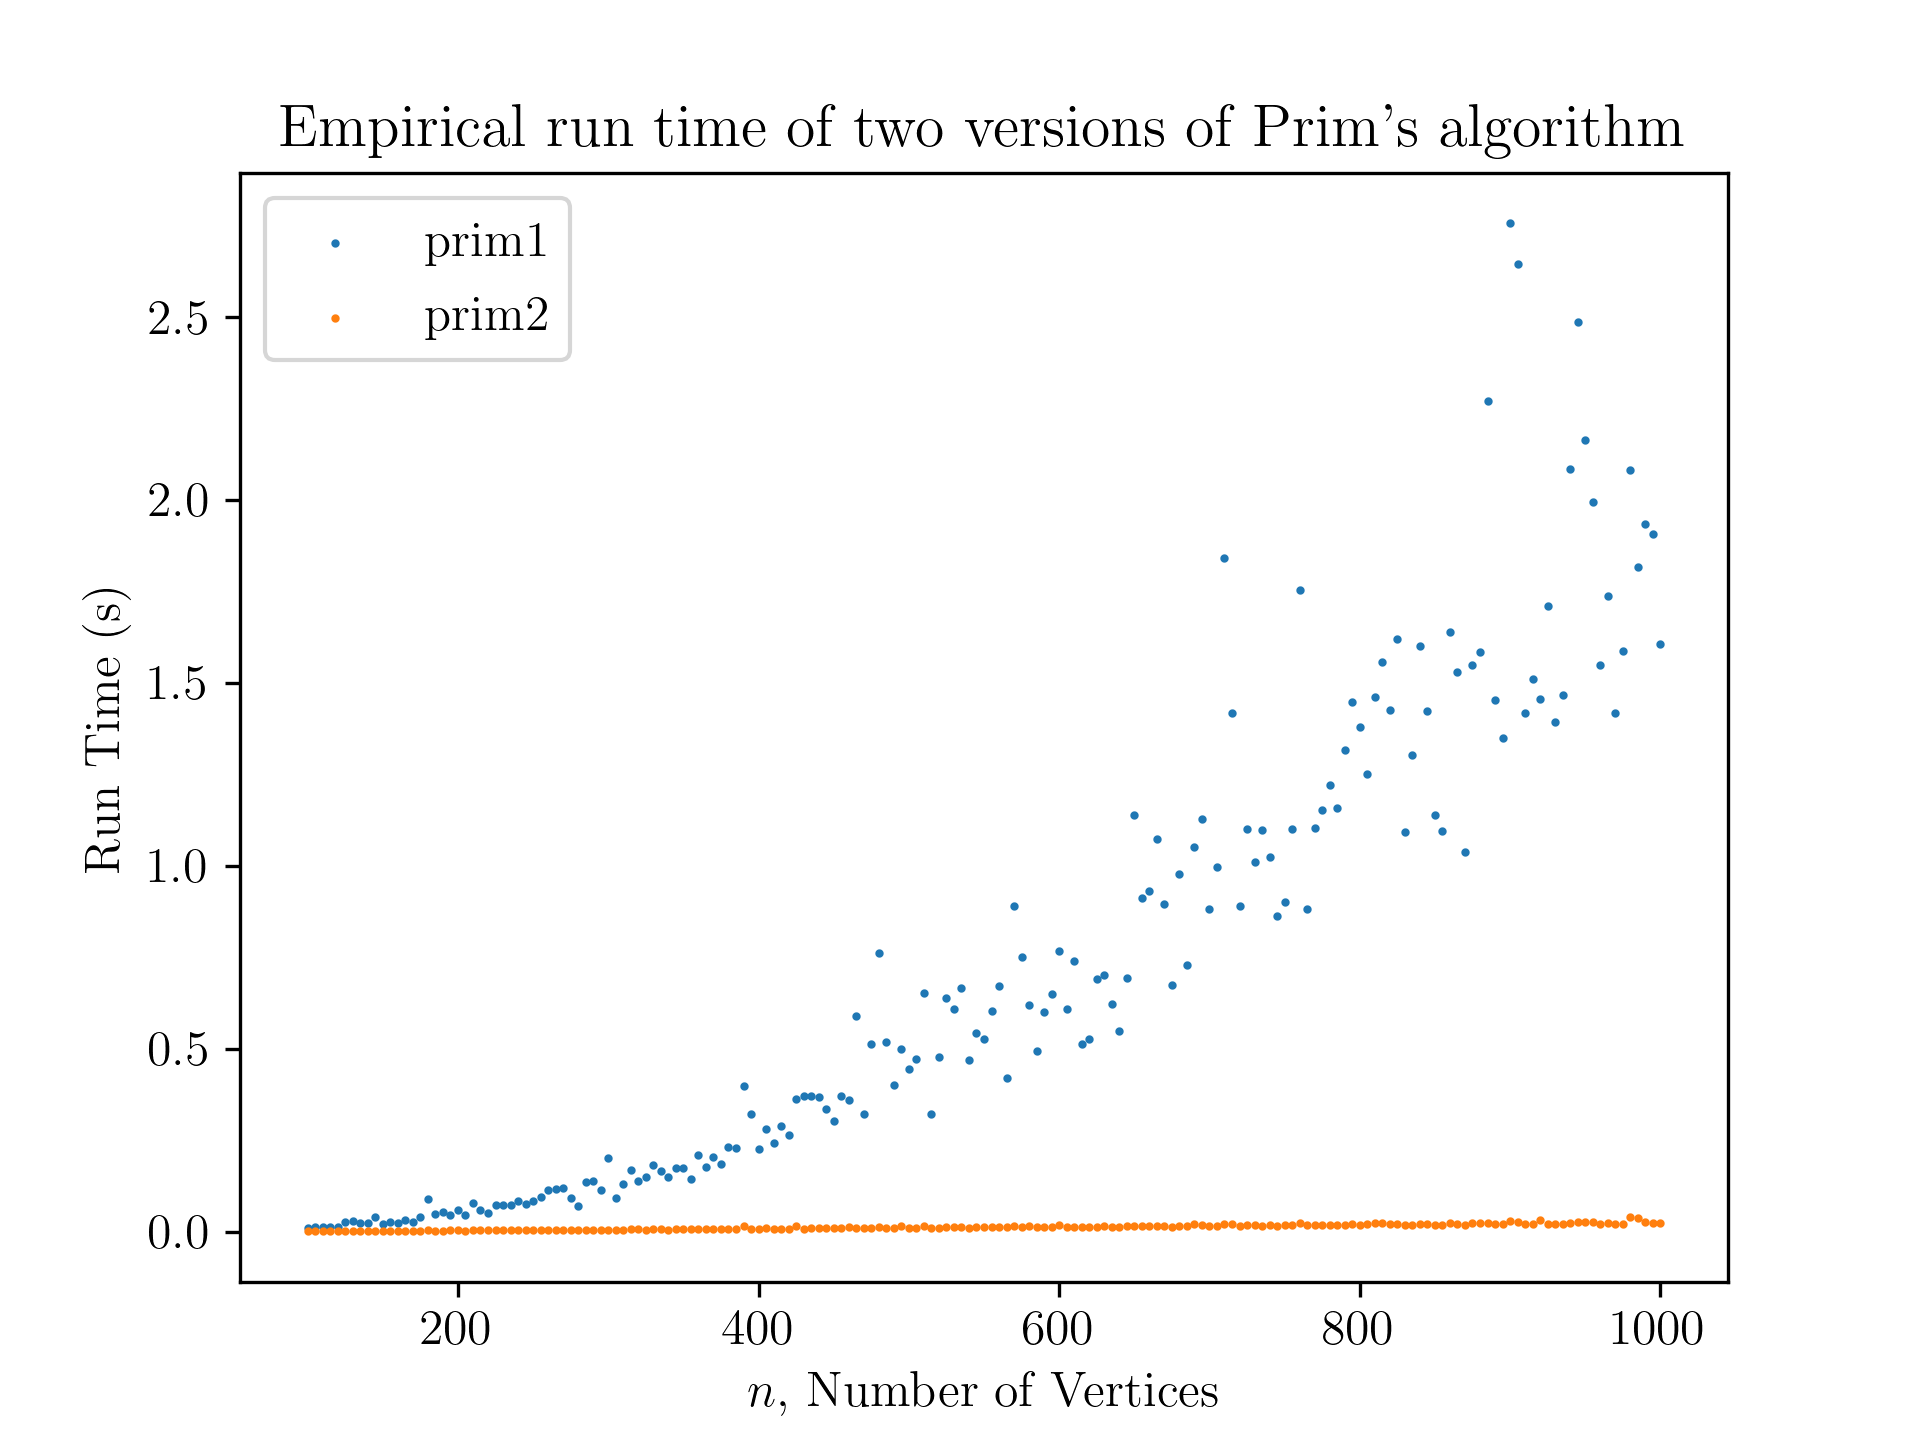
\includegraphics[width=0.8\linewidth]{comp} 
  \caption{Comparison of Prim v1 and v2}
  \label{fig:comp}
\end{figure}

To get a better understanding of the scale of growth for both versions of Prim's
MST algorithm, the two sets of empirical timing data are transformed and
visualized on different plots. Prim v1 run time is plotted on logarithmic axes
in Figure \ref{fig:v1log}. The linear regression on the transformed data yields
a slope close to 2 with a high coefficient of determination, indicating Prim v1
grows on the scale of \(\mathcal{O}(n^2)\). The graph for Prim v2 in Figure
\ref{fig:comp} is rather compressed along the y-axis due to the higher order of
growth of Prim v1. Figure \ref{fig:v2} is an isolated view of Prim v2 run time.
Since Prim v2 is expected to have a linearithmic run time, a plot of Prim v2 run
time normalized by the graph (input) size is also included, as shown in Figure
\ref{fig:v2norm}. Even though there are significant fluctuations in the plotted
data set, a rough trend of logarithmic growth is observed. Thus, our expectation
on Prim v2 run time is confirmed.
\begin{figure}[h]
  \centering
  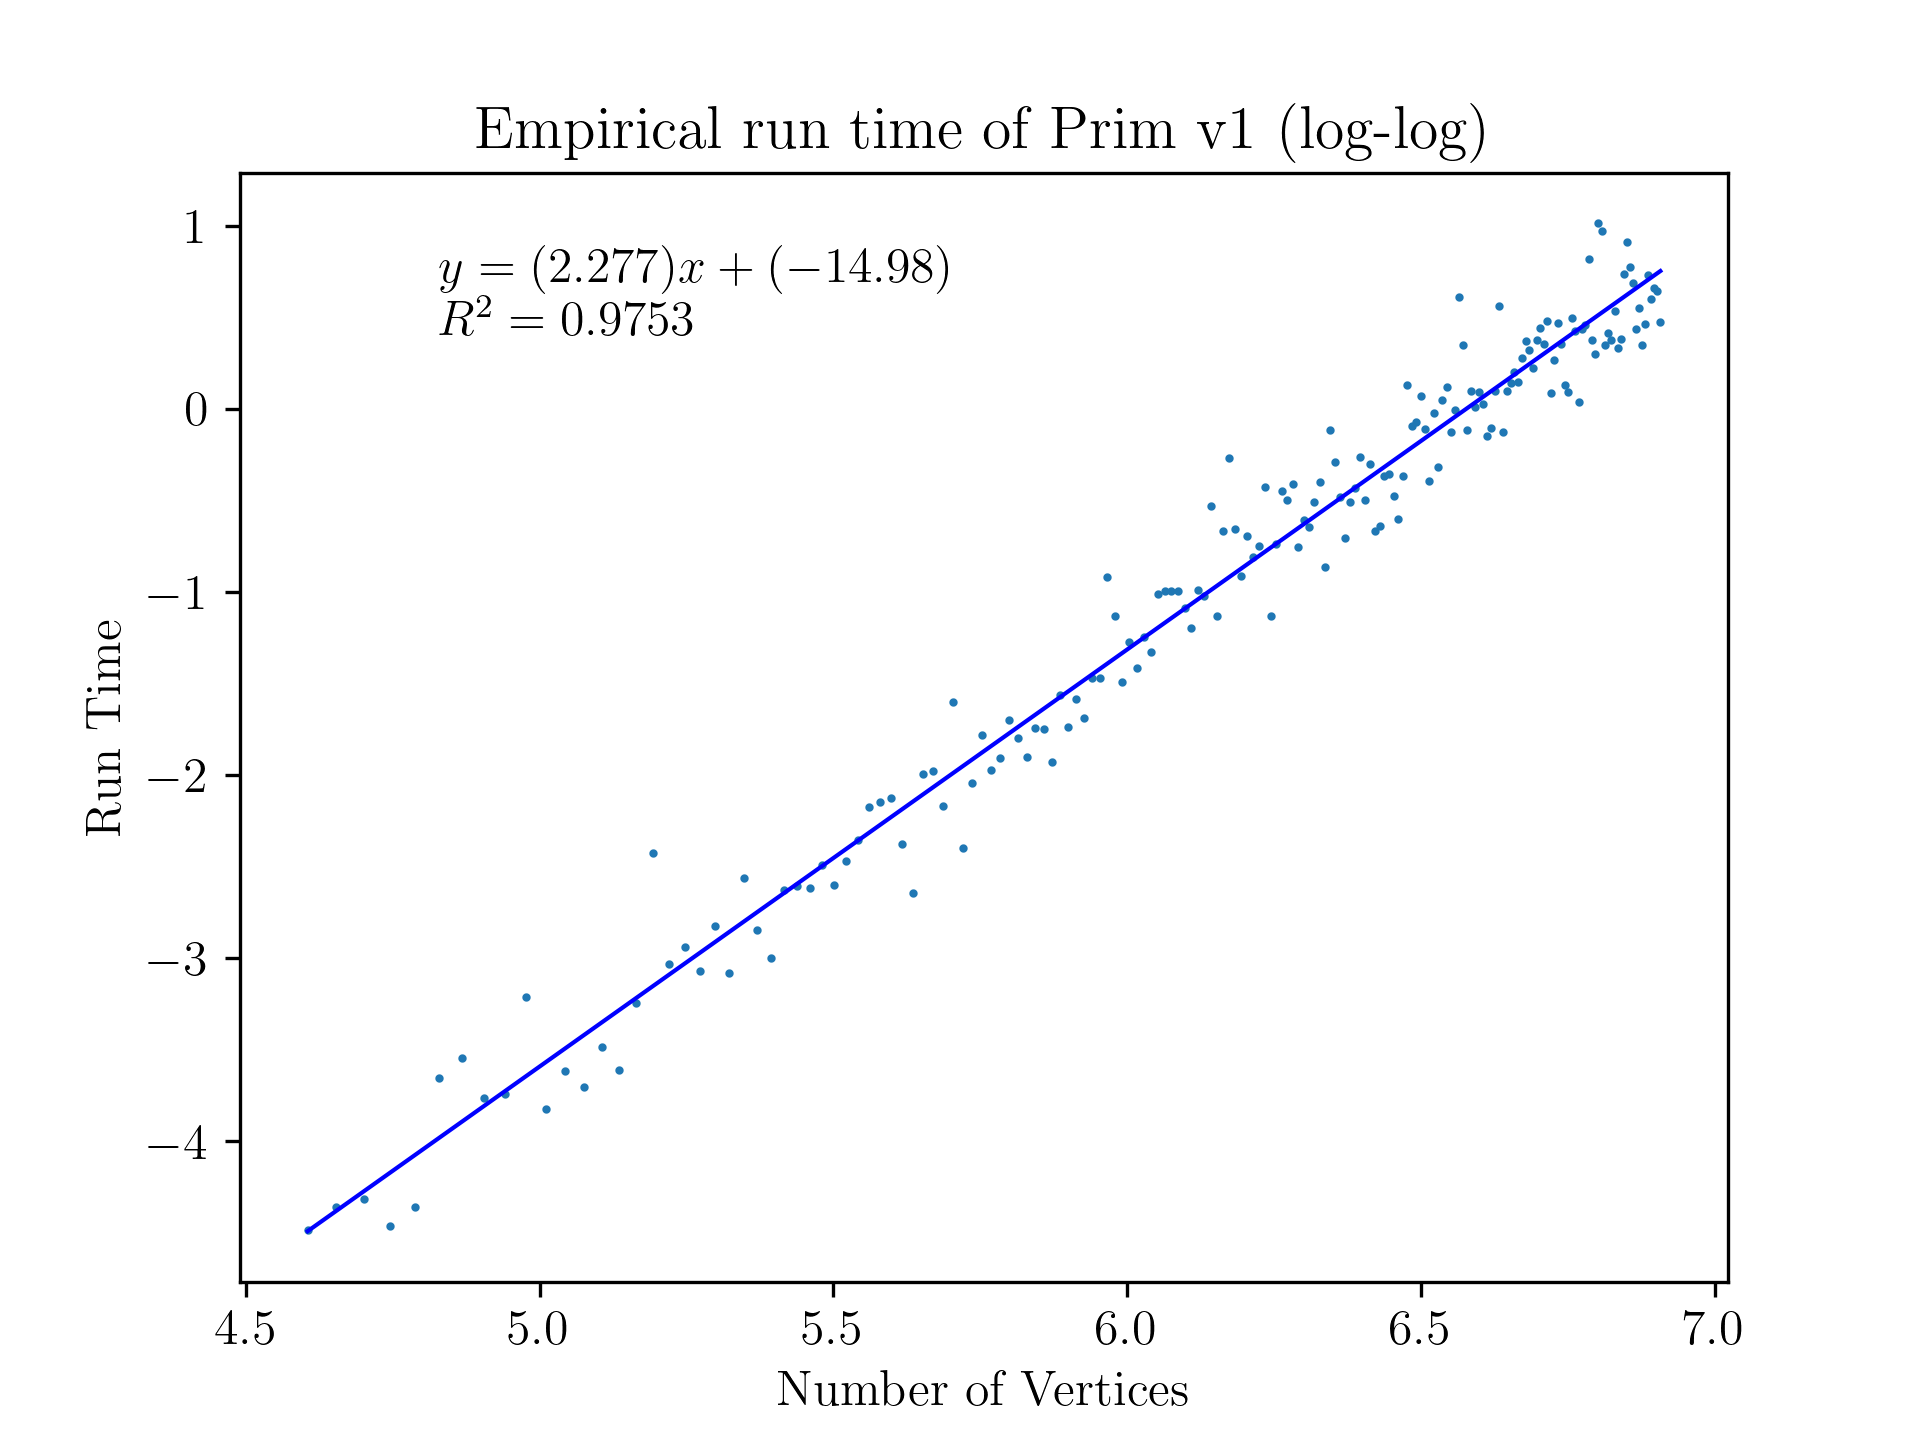
\includegraphics[width=0.8\linewidth]{v1log} 
  \caption{Log-log plot of Prim v1 run time}
  \label{fig:v1log}
\end{figure}
\begin{figure}[h]
  \centering
  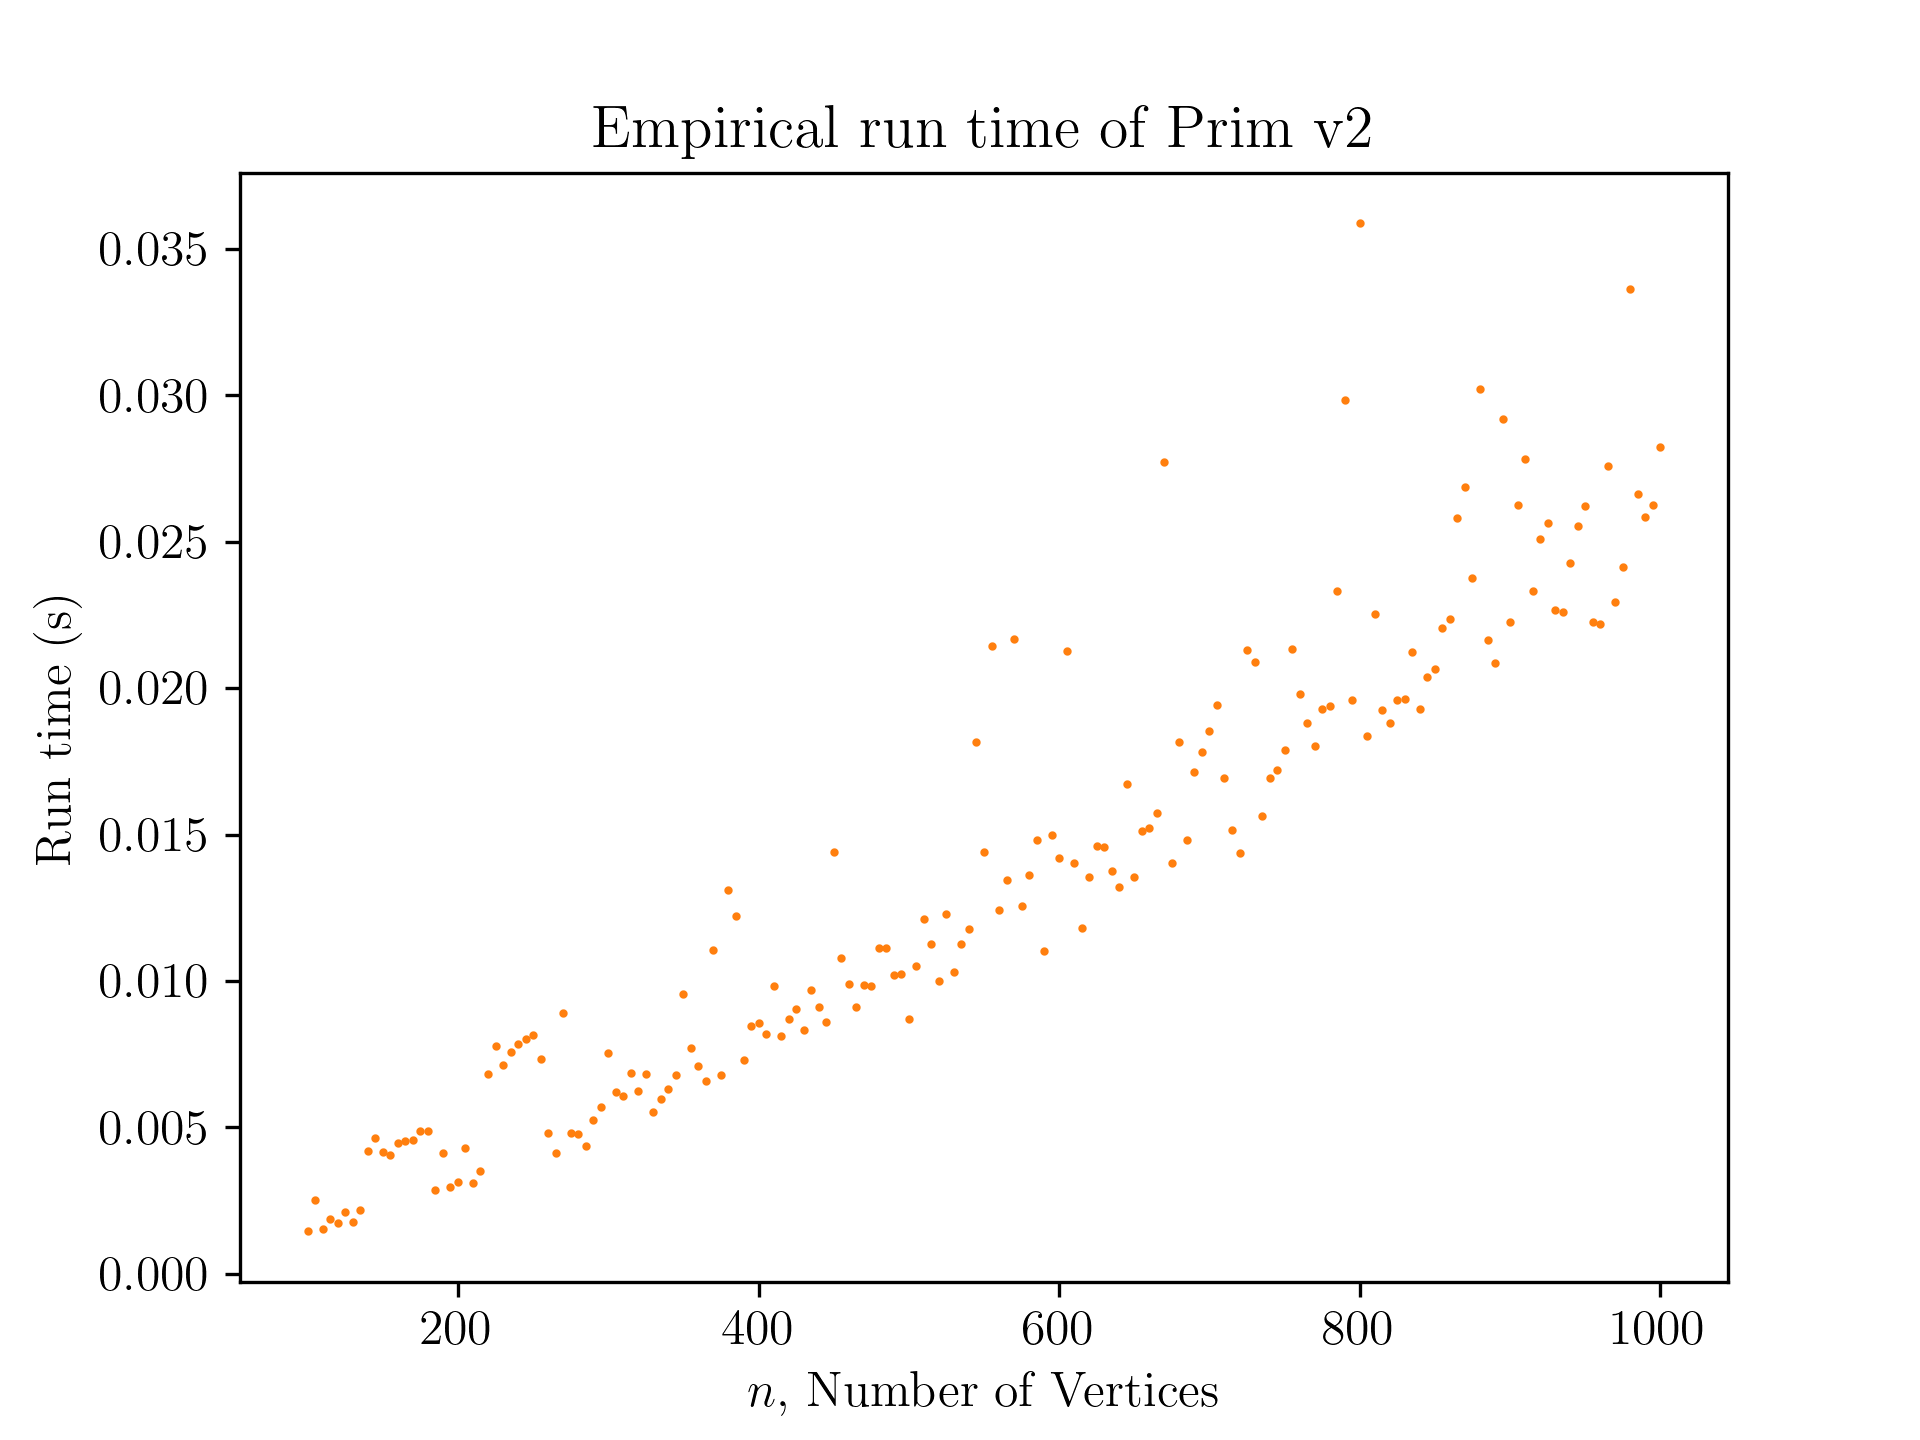
\includegraphics[width=0.8\linewidth]{v2} 
  \caption{Prim v2 run time}
  \label{fig:v2}
\end{figure}
\begin{figure}[h]
  \centering
  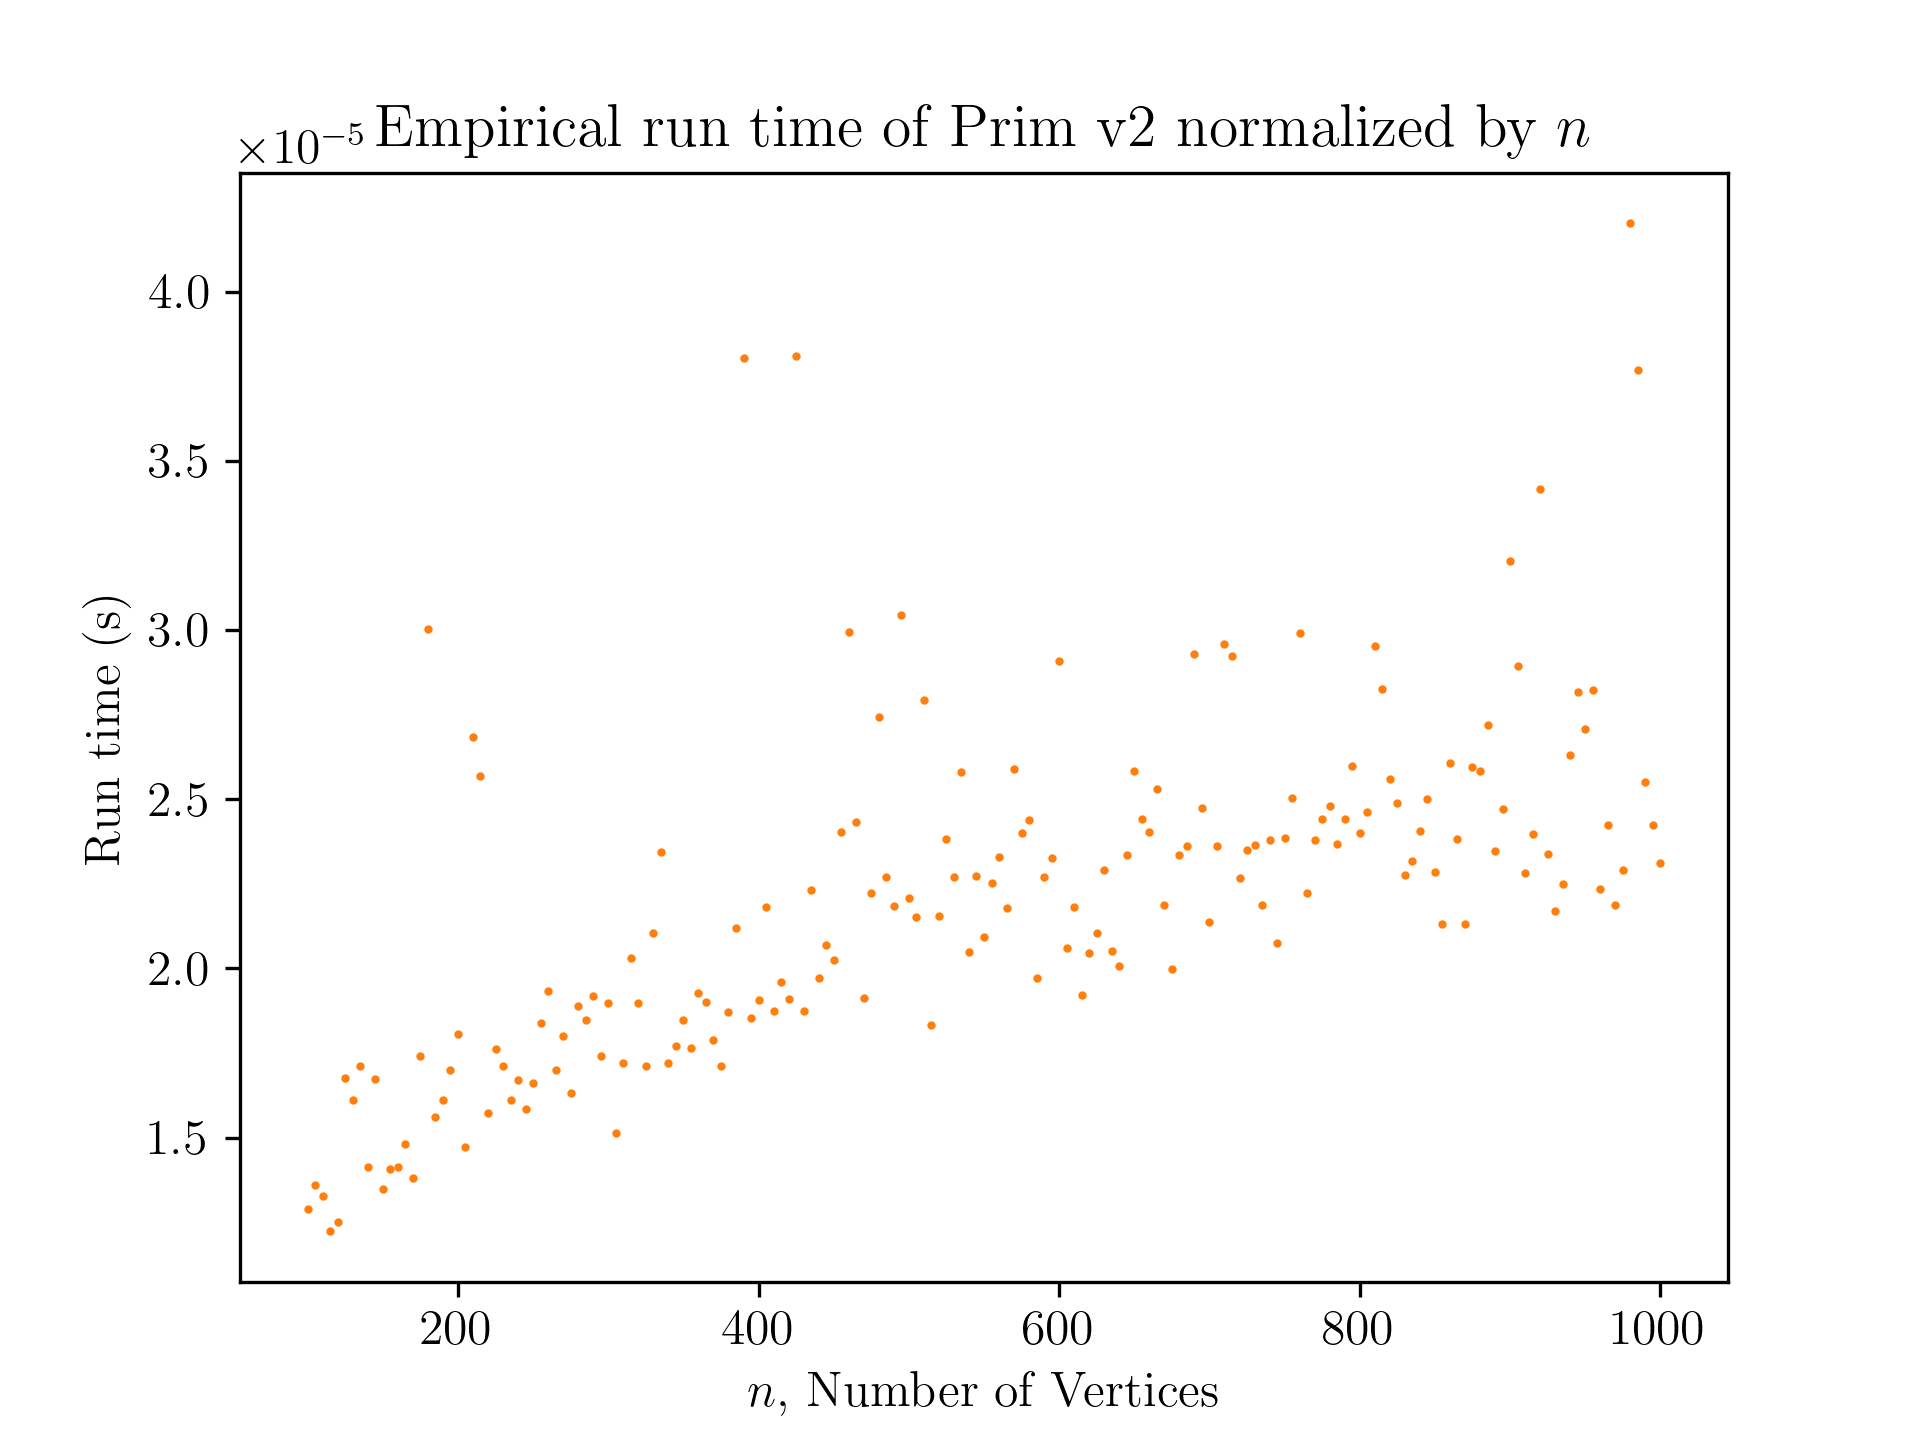
\includegraphics[width=0.8\linewidth]{v2norm} 
  \caption{Prim v2 normalized run time}
  \label{fig:v2norm}
\end{figure}

In our particular implementations of the two versions of Prim's algorithm, v1
mainly differs from v2 by the way of finding the minimum out-going edge of the
set of nodes in the MST. V1 uses a linear search for the minimum weighted edge
whenever the MST expands by one node, while v2 keeps track of a list of all the
out-going edges it discovers. Such list is maintained in a heap structure which
offers a \(\mathcal{O}(1)\) minimum query. The rest of the implementation
details are similar between the two versions. Therefore, Prim v2 is strictly a
more efficient implementation of Prim's algorithm which is accelerated by a heap
data structure.

\end{document}
